\documentclass[12pt]{article}

\usepackage[utf8]{inputenc}
\usepackage[francais]{babel}
\usepackage{tikz}
\usepackage{amsmath}
\usepackage{pgfgantt}
\usepackage{graphicx}
\usepackage{float}
\usepackage{verbatim}

\newcommand{\mmax}{\ensuremath{\operatorname{max}}}
\newcommand{\mpred}{\ensuremath{\operatorname{PRED}}}

\title{MIS 7 : Sujet d'étude n$^\circ$2}
\author{Merwan Achibet\\Université du Havre}
\date{}

\begin{document}

\maketitle

\section{Problème 1}

\subsection{Dates au plus tôt}

\underline{$b_1$}

$1$ n'a pas de prédécesseur donc $b_1 = 0$. \\

\underline{$b_2$}

$2$ a un seul prédécesseur (1), donc $b_2 = b_1 + p_1 = 0 + 3 = 3$ \\

\underline{$b_3$}

$3$ a un seul prédécesseur (1), donc $b_3 = b_1 + p_1 = 0 + 3 = 3$ \\

\underline{$b_4$}

$4$ a un seul prédécesseur (1), donc $b_4 = b_1 + p_1 = 0 + 3 = 3$ \\

\underline{$b_5$}

$5$ a trois prédécesseurs (2, 3 et 4), on choisit parmi eux $s$ tel
que $b_s + p_s + c_{s5}$ soit maximum.\\
pour 2 : $b_2 + p_2 + c_{25} = 3 + 3 + 2 = 8$\\
pour 3 : $b_3 + p_3 + c_{35} = 3 + 5 + 3 = 11$\\
pour 4 : $b_4 + p_4 + c_{45} = 3 + 3 + 1 = 7$\\
on prend donc $s = 3$.
\begin{align*}
  b_5 &= \mmax(b_S + p_s, \mmax_{i \in \mpred(5) - \{s\}}(b_i + p_i + c_{i5}))\\
  &= \mmax(3 + 5, \mmax(3 + 3 + 2, 3 + 3 + 1))\\
  &= 8
\end{align*}

\underline{$b_6$}

$6$ a deux prédécesseurs (3 et 4), on choisit parmi eux $s$ tel
que $b_s + p_s + c_{s6}$ soit maximum.\\
pour 3 : $b_3 + p_3 + c_{36} = 3 + 5 + 2 = 10$\\
pour 4 : $b_4 + p_4 + c_{46} = 3 + 3 + 1 = 7$\\
on prend donc $s = 3$.
\begin{align*}
  b_6 &= \mmax(b_S + p_s, \mmax_{i \in \mpred(6) - \{s\}}(b_i + p_i + c_{i6}))\\
  &= \mmax(3 + 5, 3 + 3 + 1)\\
  &= 8
\end{align*}

\underline{$b_7$}

$7$ a deux prédécesseurs (5 et 6), on choisit parmi eux $s$ tel
que $b_s + p_s + c_{s7}$ soit maximum.\\
pour 5 : $b_5 + p_5 + c_{57} = 8 + 4 + 1 = 13$\\
pour 6 : $b_6 + p_6 + c_{67} = 8 + 3 + 1 = 12$\\
on prend donc $s = 5$.
\begin{align*}
  b_7 &= \mmax(b_S + p_s, \mmax_{i \in \mpred(7) - \{s\}}(b_i + p_i + c_{i7}))\\
  &= \mmax(8 + 4, 8 + 3 + 1)\\
  &= 12
\end{align*}

Au final, on obtient les bornes au plus tôt suivantes :

\begin{figure}[H]
  \centering

  \begin{tabular}{|l|c|c|c|c|c|c|c|}
    \hline
    \textbf{X} & 1 & 2 & 3 & 4 & 5 & 6 & 7 \\
    \hline
    \textbf{\mpred(X)} & 0 & 3 & 3 & 3 & 8 & 8 & 12 \\
    \hline
  \end{tabular}

\end{figure}

\subsection{Diagramme de Gantt}

On construit un graphe critique contenant les arcs $(i,j)$ tels que
$b_i + p_i + c_{ij} > b_j$.\\

\underline{arc (1,2)}

$b_1 + p_1 + c_{12} = 0 + 3 + 1 = 4 > b_2 = 3$ Donc on le conserve\\

\underline{arc (1,3)}

$b_1 + p_1 + c_{13} = 0 + 3 + 2 = 5 > b_3 = 3$ Donc on le conserve\\

\underline{arc (1,4)}

$b_1 + p_1 + c_{14} = 0 + 3 + 1 > b_4 = 3$ Donc on le conserve\\

\underline{arc (2,5)}

$b_2 + p_2 + c_{25} = 3 + 3 + 2 = b_5 = 8$ Donc on le conserve\\

\underline{arc (3,5)}

$b_3 + p_3 + c_{35} = 3 + 5 + 3 > b_5 = 8$ Donc on le conserve\\

\underline{arc (3,6)}

$b_3 + p_3 + c_{36} = 3 + 5 + 2 > b_5 = 8$ Donc on le conserve\\

\underline{arc (4,5)}

$b_4 + p_4 + c_{45} = 3 + 3 + 1 < b_5 = 8$ Donc on ne le conserve pas\\

\underline{arc (4,6)}
arc(4, 6)

$b_4 + p_4 + c_{46} = 3 + 3 + 1 < b_6 = 8$ Donc on ne le conserve pas\\

\underline{arc (5,7)}

$b_5 + p_5 + c_{57} = 8 + 4 + 1 > b_7 = 12$ Donc on le conserve\\

\underline{arc (6,7)}

$b_6 + p_6 + c_{67} = 8 + 3 + 1 = b_7 = 12$ Donc on ne le conserve pas\\

Le graphe critique est donc :

\begin{figure}[H]

  \centering

  \begin{tikzpicture}
    \node[circle,draw] (1) {$1$}
    child {node[circle,draw] (2) {$2$}}
    child {node[circle,draw] (3) {$3$}
      child {node[circle,draw] (5) {$5$}
        child {node[circle,draw] (7) {$7$}}
      }
      child {node[circle,draw] (6) {$6$}}
    }
    child {node [circle,draw] (4) {$4$}};
  \end{tikzpicture}

\end{figure}

\'A partir du graphe critique, on obtient le diagramme de Gantt
suivant :

%% \begin{ganttchart}[vgrid]{14}
%%   \gantttitle{Ordonnancement optimal}{14} \\
%%   \gantttitlelist{1,...,14}{1} \\
%%   \ganttbar{P1}{1}{3}
%%   \ganttbar{}{4}{6} \\
%%   \ganttbar{P2}{1}{3}
%%   \ganttbar{}{4}{8}
%%   \ganttbar{}{9}{12}
%%   \ganttbar{}{13}{14} \\
%%   \ganttbar{P3}{1}{3}
%%   \ganttbar{}{4}{8}
%%   \ganttbar{}{9}{11} \\
%%   \ganttbar{P4}{1}{3}
%%   \ganttbar{}{4}{6}
%% \end{ganttchart}

\begin{figure}[H]
  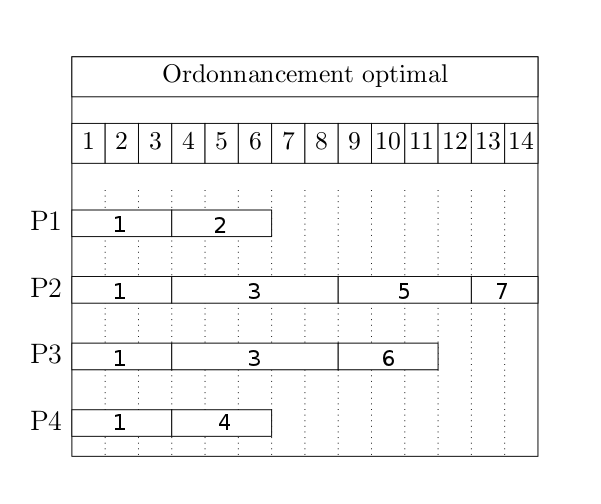
\includegraphics[width=14cm]{gantt.png}
\end{figure}

\newpage

\section{Problème 2}

\verbatiminput{pseudocode.txt}

Dans cet algorithme, le processeur maître ne réalise pas de calcul
mais répartit les données sur les quatres processeurs
esclaves. Puisqu'il y a 4 processeurs et que la matrice est de
dimension 8, on envoie deux lignes de A à chaque processeur. Par
exemple, le processeur 1 va traîter les ligne 1 et 2 tandis que le
processeur 2 va traîter les lignes 3 et 4.

Après chaque série de calcul, les processeurs esclaves envoient leurs
deux valeurs de $x$ aux autres. De cette façon, les solutions locales
de chaque P sont continuellement mises à jour.

Le test de convergence est effectué de façon décentralisée dans chaque
processeur esclave. Une fois qu'un processeur a convergé, il envoie
son résultat au processeur maître qui affiche le résultat final
lorsque tous ses esclave ont convergé.

Le graphe suivant illustre les premières itérations de l'algorithme.

\begin{figure}[H]

  \centering

  \begin{tikzpicture}

    \node[draw,circle] (P0) at (0,0) {P0};

    \node[draw,circle] (P1_1) at (3,3) {P1};
    \node[draw,circle] (P2_1) at (3,1) {P2};
    \node[draw,circle] (P3_1) at (3,-1) {P3};
    \node[draw,circle] (P4_1) at (3,-3) {P4};

    \path (P0) edge[->] (P1_1);
    \path (P0) edge[->] (P2_1);
    \path (P0) edge[->] (P3_1);
    \path (P0) edge[->] (P4_1);

    \node[draw,circle] (P1_2) at (6,3) {P1};
    \node[draw,circle] (P2_2) at (6,1) {P2};
    \node[draw,circle] (P3_2) at (6,-1) {P3};
    \node[draw,circle] (P4_2) at (6,-3) {P4};

    \path (P1_1) edge[->] (P2_2);
    \path (P1_1) edge[->] (P3_2);
    \path (P1_1) edge[->] (P4_2);
    \path (P2_1) edge[->] (P1_2);
    \path (P2_1) edge[->] (P3_2);
    \path (P2_1) edge[->] (P4_2);
    \path (P3_1) edge[->] (P1_2);
    \path (P3_1) edge[->] (P2_2);
    \path (P3_1) edge[->] (P4_2);
    \path (P4_1) edge[->] (P1_2);
    \path (P4_1) edge[->] (P2_2);
    \path (P4_1) edge[->] (P3_2);

    \node (P1_3) at (9,3) {};
    \node (P2_3) at (9,1) {};
    \node (P3_3) at (9,-1) {};
    \node (P4_3) at (9,-3) {};

    \path (P1_2) edge[dashed] (P2_3);
    \path (P1_2) edge[dashed] (P3_3);
    \path (P1_2) edge[dashed] (P4_3);
    \path (P2_2) edge[dashed] (P1_3);
    \path (P2_2) edge[dashed] (P3_3);
    \path (P2_2) edge[dashed] (P4_3);
    \path (P3_2) edge[dashed] (P1_3);
    \path (P3_2) edge[dashed] (P2_3);
    \path (P3_2) edge[dashed] (P4_3);
    \path (P4_2) edge[dashed] (P1_3);
    \path (P4_2) edge[dashed] (P2_3);
    \path (P4_2) edge[dashed] (P3_3);

  \end{tikzpicture}

\end{figure}

\end{document}
